\documentclass[12pt,a4paper]{article}
\usepackage{graphicx}
\graphicspath{{./figures/latexpdfsvg/}{./figures/svg/}{./figures/eps/}{./figures/pdf/}{./figures/png/}{./figures/latexpdf/}} 

\usepackage{amsmath,amssymb,amsfonts,amsthm}
\usepackage{hyperref}
\usepackage{spverbatim}
\usepackage{listings} 
 \lstloadlanguages{Matlab} %Other languages are available, see manual, you should select the correct language
 \lstset{
   basicstyle=\ttfamily, 
   breaklines=true, 
   columns=fixed 
  }

%% Tests of the difficult packages
%\usepackage{titlesec}
\usepackage{tikz,tikz-3dplot,pgfplots}
\usepackage{cleveref}
\usepackage{MnSymbol}
\usepackage{xcolor}
\usepackage{framed}

\newtheorem{proposition}{Proposition}[section]
\newtheorem*{example*}{Example}
\theoremstyle{definition}
\newtheorem{definition}[proposition]{Definition}
\theoremstyle{remark}
\newtheorem{remark}[proposition]{Remark}
\newtheorem{example}[proposition]{Example}
\newcommand{\bvec}[1]{\mathrm{\mathbf{#1}}}
\newcommand{\cvec}[2]{\begin{pmatrix} #1 \\ #2 \end{pmatrix}} 
\newcommand{\vmod}[1]{{\lvert {#1} \rvert}}
\newcommand{\R}{\mathbb{R}}

%%%%%%%%%%%%%%%%%%%%%%%%%%%%%%%%%%%%%%%%%%%%%%%%%%%%%
%% Define front matter
\title{MArefSetup}
\author{Emma Cliffe}
\date{2017}

\begin{document}

\maketitle

\tableofcontents

\section*{Test}

This section should be in the contents page for the PDF but not the web or word. 

\section{Quadratic equations}

A quadratic equation is an equation with the form \(ax^2 + bx + c = 0\) where \(x\) represents an unknown and \(a\), \(b\) and \(c\) are known numbers with \(a \neq 0\). 

\subsection{Solutions to a quadratic equation}

A solution to a quadratic equation is a value of \(x\) such that the equation balances. The solutions to quadratic equations can be found by using the quadratic formula: 
\begin{equation}
\label{quadform}
x = \frac{-b \pm \sqrt{b^2-4ac}}{2a}.
\end{equation}

\begin{example*}
For instance, the solutions to \(x^2 + 2x -3 = 0\) are:
%% We can't leave the first column of an array-like equation environment empty
%% JAWS is unable to locate the row. Adding in white space will not alter 
%% layout. 
\begin{align*}
x &= \frac{-2 \pm \sqrt{2^2-4\times 1 \times -3}}{2 \times 1}\\
\,&= \frac{-2 \pm \sqrt{4+12}}{2}\\
\,&= \frac{-2 \pm \sqrt{16}}{2}\\
\,&= \frac{-2 \pm 4}{2}
\end{align*} 
Hence, \(x = 1\) or \(x = -3\).  
\end{example*}

\subsection{The discriminant}

\begin{definition}[Discriminant]
The \emph{discriminant} of a quadratic equation with coefficients \(a, b, c \in \mathbb{R}\) is:
\[
\Delta = b^2 - 4ac.
\]
\end{definition}

\begin{remark}
{\bf Note that} this is the expression beneath the square root symbol in the quadratic formula (\cref{quadform}).
\end{remark}

We can use the discriminant to determine the number of real roots of a quadratic equation. The number depends on the value of \(\Delta\) as in table \cref{Distable}.
\begin{table}[!h]
\begin{center}
\begin{tabular}{|l|l|}
\hline
Value of \(\Delta\) & Real roots \\
\hline
\(\Delta > 0\) & Two, distinct\\
\(\Delta = 0\) & One, repeated\\
\(\Delta < 0\) & Zero\\
\hline
\end{tabular}
\end{center}
\caption{Number of real roots of a quadratic equation, given the discriminant}
\label{Distable}
\end{table}

%Footnotes are 'lost' in the word document format - they are links into the html version
Figure \cref{DisFig} shows an example of each possibility\footnote{The image is due to Olin, CC-BY-AS 3.0 downloaded from \href{https://commons.wikimedia.org/wiki/File:Quadratic_eq_discriminant.svg}{Wikimedia Commons}}.
\begin{figure}[!h]
\begin{center}
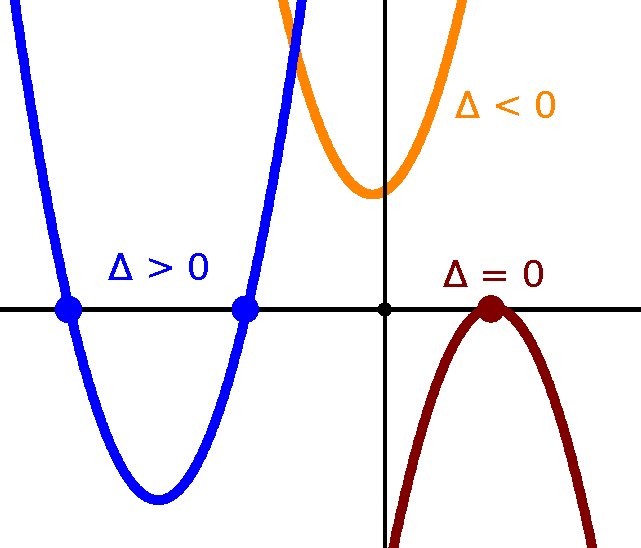
\includegraphics[width=0.5\textwidth]{Quadratic_eq_discriminant.pdf}
\end{center}
\caption{Examples of quadratic functions with zero, one and two real roots.}
\label{DisFig}
\end{figure}


\newpage
\section{The scalar product}

Consider two vectors \(\bvec{a}\) and \(\bvec{b}\) drawn so their tails are at the same point. 
\begin{figure}[!h]
\begin{center}
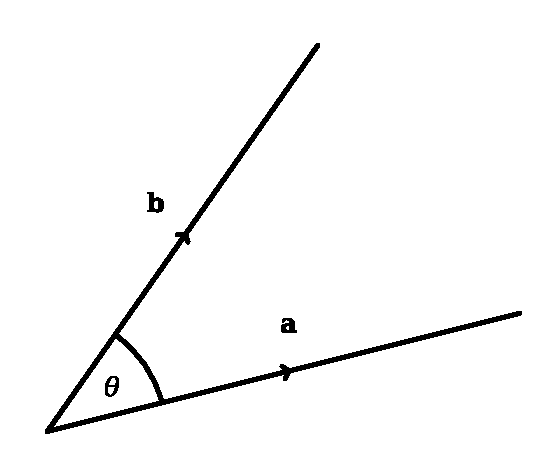
\includegraphics[width=0.6\textwidth]{vectors.eps}
\end{center}
\caption{Two vectors with angle between them.}
\label{vectors}
\end{figure}

We define the scalar product of \(\bvec{a}\) and \(\bvec{b}\) as follows. 

\begin{definition}[Scalar product]
The \emph{scalar product} of \(\bvec{a}\) and \(\bvec{b}\) is
%% We must use \lvert and \rvert to ensure that they are matched
%% in the web rendering. \left| and \right| will not be read
%% aloud correctly. | and | may differ in size.  
\[
\bvec{a}\cdot \bvec{b} = \lvert\bvec{a}\rvert \lvert\bvec{b}\rvert \cos \theta
\]
where
\begin{itemize}
\item \(\lvert\bvec{a}\rvert\) is the modulus of \(\bvec{a}\),
\item \(\lvert\bvec{b}\rvert\) is the modulus of \(\bvec{b}\), and
\item \(\theta\) is the angle between \(\bvec{a}\) and \(\bvec{b}\). 
\end{itemize}
\end{definition}

\begin{remark}
It is important to use the dot symbol for the scalar product (also called the dot product). You must not use a \(\times\) symbol as this denotes the vector product which is defined differently. 
\end{remark}

\begin{example}
Let 
\[
\bvec{a} = \cvec{2}{2} \quad \text{and} \quad \bvec{b} = \cvec{4}{0}.
\]
The angle between these vectors is \(\theta = {45}^{\circ}\). Then \(\vmod{\bvec{a}} = \sqrt{8} \) and \(\vmod{\bvec{b}} = 4\). So, 
\begin{align*}
\bvec{a} \cdot \bvec{b} = \cvec{2}{2}\,\cdot\, \cvec{4}{0} &= \vmod{\bvec{a}}\vmod{\bvec{b}}\cos\theta \\
\,&= \sqrt{8} \times 4 \times \cos {45}^{\circ} \\
\,&= 4\sqrt{8}\times \frac{1}{\sqrt{2}} = 4\frac{\sqrt{8}}{\sqrt{2}} = 4\sqrt{4} = 8.
\end{align*} 
Note that the result is a scalar, not a vector. 
\end{example}

\subsection{Vectors in cartesian form}

When vectors are given in cartesian form there is an alternative formula for calculating the scalar product. 
\begin{proposition}
If \(\bvec{a} = a_1\bvec{i} + a_2\bvec{j}\) and \(\bvec{b} = b_1\bvec{i} + b_2\bvec{j}\) then
\[
\bvec{a} \cdot \bvec{b} = a_1b_1 + a_2b_2.
\]
\end{proposition}

\begin{proof}
Consider the vector \(\bvec{b} - \bvec{a} = \cvec{b_1 - a_1}{b_2 - a_2}\). The modulus of this is
\[
\vmod{\bvec{b} - \bvec{a}} = \sqrt{(b_1 - a_2)^2 + (b_2 - a_2)^2}.
\] 
Note from figure \cref{triangle} that the vectors \(\bvec{a}\), \(\bvec{b}\) and \(\bvec{b}-\bvec{a}\) form a triangle: 
\begin{figure}[!h]
\begin{center}
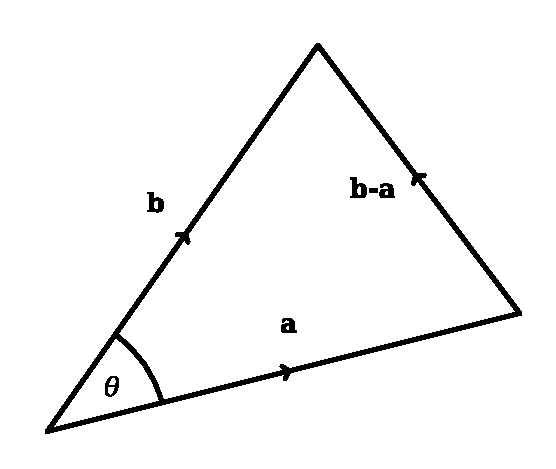
\includegraphics[width=0.6\textwidth]{triangle.eps}
\end{center}
\caption{A triangle is formed by two vectors and their difference.}
\label{triangle}
\end{figure}

Let \(\theta\) denote the angle between \(\bvec{a}\) and \(\bvec{b}\). Then, the cosine rule yields:
%% When squaring the modulus we need to place the entire item
%% to be square in braces otherwise some readers interpret the
%% | as divides.
\begin{equation}
\label{cosrule}
{\vmod{\bvec{b}-\bvec{a}}}^2 = {\vmod{\bvec{a}}}^2 + {\vmod{\bvec{b}}}^2 - 2\vmod{\bvec{a}}\vmod{\bvec{b}}\cos\theta. 
\end{equation} 
Substituting the definition of the scalar product of \(\bvec{a}\) and \(\bvec{b}\) into equation \cref{cosrule} gives:
\[
{\vmod{\bvec{b}-\bvec{a}}}^2 = {\vmod{\bvec{a}}}^2 + {\vmod{\bvec{b}}}^2 - 2\left(\bvec{a}\cdot \bvec{b}\right).
\] 
Rearranging:
\[
\left(\bvec{a}\cdot \bvec{b}\right) = \frac{1}{2}\left({\vmod{\bvec{a}}}^2 + {\vmod{\bvec{b}}}^2 - {\vmod{\bvec{b}-\bvec{a}}}^2\right).
\]
Writing this in terms of components produces:
\begin{align*}
\left(\bvec{a}\cdot \bvec{b}\right) &= \frac{1}{2}\left(a_1^2 + a_2^2 + b_1^2 + b_2^2 - (b_1 - a_1)^2 - (b_2 - a_2)^2\right)\\
\,&=\frac{1}{2}\left(a_1^2 + a_2^2 + b_1^2 + b_2^2 - b_1^2 + 2b_1a_1 - a_1^2 - b_2^2 + 2b_2a_2 - a_2^2\right)\\
\,&=\frac{1}{2}\left(2b_1a_1 + 2b_2a_2\right)\\
\,&=a_1b_1 + a_2b_2
\end{align*}
as required. 
\end{proof}

\begin{example}
Consider again the vectors
\[
\bvec{a} = \cvec{2}{2} \quad \text{and} \quad \bvec{b} = \cvec{4}{0}.
\]
Calculating the scalar product using the components:
\[
\bvec{a} \cdot \bvec{b} = a_1b_1 + a_2b_2 = 2\times 4 + 2\times 0 = 8. 
\]

Note that if we are given vectors in this form, the scalar product may be used to calculate the angle between them. Since \(\bvec{a} \cdot \bvec{b} = 8\) and we have:
\begin{align*}
\vmod{\bvec{a}} &= \sqrt{8}\\
\vmod{\bvec{b}} &= 4.
\end{align*}
Hence,
\begin{align*}
8 = \bvec{a} \cdot \bvec{b} &= \vmod{\bvec{a}}\vmod{\bvec{b}}\cos\theta\\
\,&= 4\sqrt{8}\cos \theta.
\end{align*}
Rearranging:
\[
\theta = \cos^{-1}\left(\frac{8}{4\sqrt{8}}\right) = {45}^{\circ}.
\]
\end{example}

\section{Using Matlab}

Two calculate the scalar product in Matlab the \spverb=dot= function is used. 

Create two vectors:
\begin{lstlisting}
> A = [4 -1 2];
> B = [2 -2 -1];
\end{lstlisting}

Calculate the scalar product:
\begin{lstlisting}
> C = dot(A,B)
    
    C = 8
\end{lstlisting}

\section{Using Tikz}

\begin{figure}[ht]
  \centering
  \tdplotsetmaincoords{70}{60}
  \begin{tikzpicture}[tdplot_main_coords]
    \draw[fill=yellow!10!white,opacity=0.3] (-4,-4,0) -- (-4,4,0) --
    (4,4,0) -- (4,-4,0) -- cycle;
    \draw
    [blue,dashed] (-1.7,-1.7,-1.7) -- (0,0,0);
    \draw [blue]
    (0,0,0)--(4,4,4); \draw[blue] (-3,-3,-3)--(-1.7,-1.7,-1.7);
    \filldraw[red] (0,0,0) node[black,above left]{$0$} circle (.5mm);
    \node[black,above left] at (3,3,3) {$V_{2}$} ;
    \node[black,right] at (4,4,0) {$V_{1}$}; 
  \end{tikzpicture}
  \caption{$\R^3$ as a direct sum of a line and a plane}
  \label{fig:dsum}
\end{figure}

\begin{figure}[htb]
  \centering
\begin{tikzpicture}[line cap=round,line join=round,>=triangle 45,x=0.3cm,y=0.3cm]
\clip(-7.92,-5.551666666666653) rectangle (7.47,6.643333333333327);
\draw [color=blue,domain=-7.92:7.47] plot(\x,{(-3.5608-6.9*\x)/-3.04});
\draw [color=blue,domain=-7.92:7.47] plot(\x,{(-8.2736--1.56*\x)/7.78});
\draw [dash pattern=on 3pt off 3pt,color=blue] (0.42281833116739825,2.1310021332417923)-- (3.46,2.74);
\draw [dash pattern=on 3pt off 3pt,color=blue] (1.957181668832602,-0.6710021332417918)-- (3.46,2.74);
\draw [fill,red] (-1.08,-1.28) circle (1.0pt) node[black,below right] {$0$};
\draw (1.6875,6.103333333333328) node[left] {$V_2$};
\draw (-7.4475,-1.6816666666666595) node {$V_1$};
\draw [fill,red] (3.46,2.74) circle (1.0pt) node[black,right] {$v$};
\draw [fill,red] (1.957181668832602,-0.6710021332417918)
circle (1.0pt)  node[black,below] {$v_1$};
\draw [fill,red] (0.42281833116739825,2.1310021332417923)
circle (1.0pt) node[left,black] {$v_2$};
\end{tikzpicture}
  \caption{$\R^2=V_1\oplus V_2$}
  \label{fig:decomp}
\end{figure}

\section{Testing pdftex graphics}

  \begin{figure}[H]
    \centering
    \def\svgwidth{0.5\columnwidth}
    \input{Semiannulus.pdf_tex}
  \end{figure}

\section{Package tests}

This should be a north east south west arrow: \(\neswarrow\) and this should be a north west south east arrow: \(\nwsearrow\). 

\begin{framed}
This is in a frame
\end{framed}

\colorlet{shadecolor}{blue!5}
\begin{shaded}
This is shaded
\end{shaded}

\end{document}
